%%
% Interação e Deteção de Partículas - MIEF
% Problema 3 - 
%
% Data: 03/11/2021


\documentclass[a4paper, 12pt]{article} % Set to article class
\usepackage[portuguese]{babel} % Set language to portuguese

\usepackage{lmodern} % Changes to a cleaner font
\usepackage{listings}
\usepackage{color}


\usepackage[T1]{fontenc} % Add support to language
\usepackage[cp1252, utf8]{inputenc} % Add support to language

\chardef\_=`_ % Add support to underscores
\usepackage{graphicx, epstopdf, rotating, % Graphics support
	array, booktabs, float, % Tables packages
	makecell, enumitem, 
	amsmath, amssymb, % Better math print
	siunitx % Plot support	
} % Add basic support

\usepackage[bookmarks, pdftex, hidelinks]{hyperref} % Add hidden bookmarks
\usepackage[margin = .75in]{geometry} % Tool to remove margins
\graphicspath{{images/}} % Add path to images folder

\renewcommand\theadfont{\bfseries} % Make table headers better
\setlength\parindent{0pt} % Remove paragraph indent
\pagestyle{plain} % Adds custom page style
\usepackage[font=small]{caption} % Change caption size

% Nome da disciplina
\def\classtitle{Interação e Deteção de Partículas}

% Nome do relatório
\def\worktitle{Problema 3 - Blindagem contra raios-$\gamma$}

% Nome do/a professor/a
\def\profname{Doutor Alexandre Lindote}

% Nome do local 
\def\worklocal{Universidade de Coimbra}

% Data do trabalho
\def\workdate{\today}

% Nome dos autores
\def\authors{
	José Nuno da Cruz Faria - 2015252736
}

% Turma
\def\classinfo{Teórica Prática, Turma PL1}

\renewcommand\thesection{\arabic{section})}

% Resize matrice lines
\makeatletter
\renewcommand*\env@matrix[1][\arraystretch]{%
  \edef\arraystretch{#1}%
  \hskip -\arraycolsep
  \let\@ifnextchar\new@ifnextchar
  \array{*\c@MaxMatrixCols c}}
\makeatother

\definecolor{clr-background}{RGB}{255,255,255}
\definecolor{clr-text}{RGB}{0,0,0}
\definecolor{clr-string}{RGB}{163,21,21}
\definecolor{clr-namespace}{RGB}{0,0,0}
\definecolor{clr-preprocessor}{RGB}{128,128,128}
\definecolor{clr-keyword}{RGB}{0,0,255}
\definecolor{clr-type}{RGB}{43,145,175}
\definecolor{clr-variable}{RGB}{0,0,0}
\definecolor{clr-constant}{RGB}{111,0,138} % macro color
\definecolor{clr-comment}{RGB}{0,128,0}

\lstdefinestyle{VS2017}{
	backgroundcolor=\color{clr-background}\ttfamily,
	basicstyle=\color{clr-text}\ttfamily, % any text
	stringstyle=\color{clr-string}\ttfamily,
	identifierstyle=\color{clr-variable}\ttfamily, % just about anything that isn't a directive, comment, string or known type
	commentstyle=\color{clr-comment}\ttfamily,
	directivestyle=\color{clr-preprocessor}\ttfamily, % preprocessor commands
	% listings doesn't differentiate between types and keywords (e.g. int vs return)
	% use the user types color
	keywordstyle=\color{clr-type}\ttfamily,
	%keywordstyle={\color{clr-constant}}\ttfamily, % you'll need to define these or use a custom language
	tabsize=4
}


\lstset{language=C++,
                style=VS2017
}


\begin{document}
	
	\begin{figure}[t] % Add logo
		\centering
		
\includegraphics[width=0.85\linewidth]{uc_fctuc}
	\end{figure}

	\vspace*{0.05\textheight}	
	\begin{table}[!htbp]
		\centering
		
		{\Huge \classtitle}\\
		
		\vspace*{0.01\textheight}
		{\Large \textbf{\worktitle}}\\
		
		\vspace*{0.02\textheight}
		{\large {\worklocal, \workdate}}
		
	\end{table}
	
	\begin{table}[H]
		\begin{center}
			{\normalsize % Mudar a fonte para mais pequena(?)
				\textbf\classinfo\\
				\emph{Prof. \profname}\\ 
				\vspace{0.0035\textheight}			
				\authors 
			}
		\end{center}
	\end{table}

	\section{Determinar a espessura de Pb necessária para reduzir a intensidade de um feixe de raios-$\gamma$ em 90\% }
	Para um feixe estreito monocromático com uma intensidade $I_0$ que atravessa um camada de material de espessura $x$ e densidade $\rho$, a intensidade do feixe emergente pode ser obtida através:

	\begin{equation}
		I = I_0 \times e^{-x\mu_m\rho}
		\label{eq:attenuation}
	\end{equation}
	onde coeficiente de atenuação mássico é $\mu_m$ do material.
	
	\paragraph{} Figura \ref{fig:attenuation} mostra o coeficiente de absorção mássico do Pb em função da energia da feixe incidente. Observa-se que para um feixe de 1 MeV, temos $\mu_m=7.102 \times 10^{-2}\ \text{cm}^2/g$.
	
	\begin{figure}[H]
		\centering
		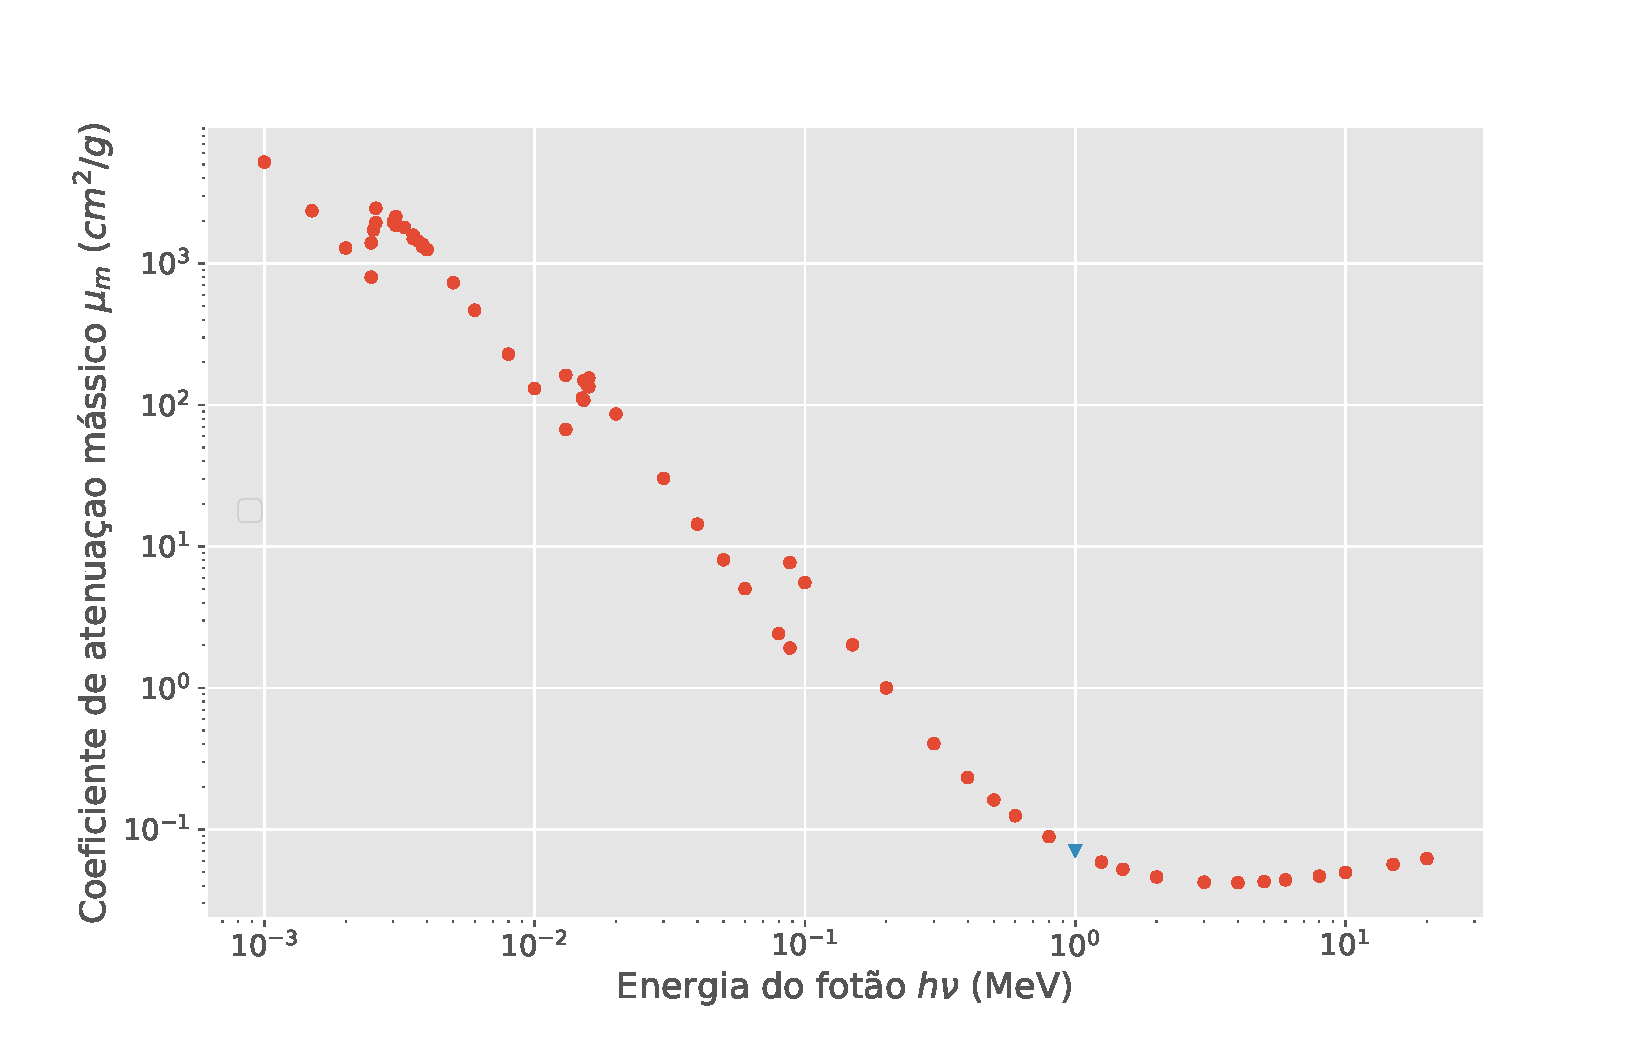
\includegraphics[width=0.6\linewidth]{u_plot.pdf}
		\caption{Coeficiente de absorção mássico do Pb em função da energia da radiação incidente. Fonte: \url{https://physics.nist.gov/PhysRefData/XrayMassCoef/ElemTab/z82.html}}
		\label{fig:attenuation}
	\end{figure}

	\paragraph{} Para determinar a espessura necessária da placa de Pb para ter uma redução de 90\% de energia no feixe incidente, usamos a equação \ref{eq:attenuation}:


	\begin{align}
		I &= I_0 \times e^{-x\mu_m\rho} \\
		\Rightarrow \frac{1}{10} &= e^{-x(7.102 \times 10^{-2})\times(11.2)}\\
		\Rightarrow x&=\frac{\ln(10)}{7.102 \times 10^{-2}\times 11.2} \approx 2.89\ \text{cm}
		\label{eq:attenuation_result}
	\end{align}

	\section{Simulador}
	O código para o simulador de Monte-Carlo foi criado em Geant4 com base no \textit{template} fornecido\footnote{\url{https://lip.pt/~alex/G4Classes/Examples/Shielding.zip}}, e encontra-se no seguinte URL: \url{https://github.com/jncfa/idp_exercices/tree/master/class4/tpc}.

	\paragraph{} Para criar o simulador é necessário adicionar implementar 3 componentes ao \textit{template}:
	
	\begin{enumerate}
		\item Geometria da Simulação: Definir a posição e orientação de cada componente a simular, \textit{i.e.} posição e orientação da placa de Pb e do detector (que no nosso caso, não representa um detector real mas sim um ``volume artificial'' usado apenas para verificar se as partículas atravessaram a placa de Pb).
		\item Gerador da Partículas Primárias: Definir quais são as partículas emitidas e as suas propriedades (\textit{i.e.} energia, posição, e orientação de cada partícula).
		\item Recolha de informação para análise: Definir um mecanismo que permita a recolha dos dados da simulação.
	\end{enumerate}

	Nas próximas secções, é explicada como é implementada cada componente.

	\subsection{Geometria da Simulação}
	Para definir a geometria da simulação, utiliza-se a classe \texttt{G4VUserDetectorConstruction}\footnote{\url{https://apc.u-paris.fr/~franco/g4doxy4.10/html/class_g4_v_user_detector_construction.html}} para definir a posição, orientação dos materiais que compõe o nosso detector e da placa de Pb.  

	\begin{lstlisting}[language=C++]
		G4Element *Pb = new G4Element("Lead", "Pb", z = 82., a = 207.2 * g / mole);
	\end{lstlisting}

	\subsection{Gerador da Partículas Primárias}
	Para definir as partículas que são geradas na simulação, utiliza-se uma classe do tipo \\\texttt{G4VUserPrimaryGeneratorAction}\footnote{\url{https://apc.u-paris.fr/~franco/g4doxy4.10/html/class_g4_v_user_primary_generator_action.html}} para definir o evento de ``geração'' de partículas. Nessa classe, é criada uma \texttt{G4ParticuleGun}\footnote{\url{https://apc.u-paris.fr/~franco/g4doxy/html/classG4ParticleGun.html}} que emite uma partícula-$\gamma$, com 1 MeV.


	\begin{lstlisting}[language=C++]
// criar uma particle gun de uma particula
G4ParticleGun particleGun = new G4ParticleGun(1);
// obter informacao das particulas gamma
G4ParticleTable *particleTable = G4ParticleTable::GetParticleTable();
G4ParticleDefinition *particle = particleTable->FindParticle("gamma");
particleGun->SetParticleDefinition(particle);
// definir posicao, orientacao e momento da particula
particleGun->SetParticleMomentumDirection(G4ThreeVector(1., 0., 0.));
particleGun->SetParticleEnergy(1.0 * MeV);
particleGun->SetParticlePosition(G4ThreeVector(-1*m, 0. * cm, 0. * cm));
	\end{lstlisting}

	\subsection{Recolha informação para análise }
	Para recolher os dados da simulação, criamos uma classe do tipo \texttt{G4UserSteppingAction}\footnote{\url{https://apc.u-paris.fr/~franco/g4doxy/html/classG4UserSteppingAction.html}} que é chamada a cada passo da iteração da simulação.

	\paragraph{} Em cada passo, o programa verifica se a partícula que está a ser seguida neste passo encontra-se no volume do detector, e verifica se é uma partícula-$\gamma$. Caso estas condições se verifiquem, as propriedades da partícula (posição e energia) são registadas no ficheiro ``Shielding\_Pb.out'', como se pode observar no código seguinte:

	\begin{lstlisting}[language=C++]
// Na inicializacao da classe..
std::ofstream bout;
bout.open("Shielding_Pb.out");
//Codigo chamado a cada passo
G4Track *thisTrack = thisStep->GetTrack();
G4VPhysicalVolume *theVolume = thisTrack->GetVolume();
const G4ParticleDefinition *thisParticle = 
	thisTrack->GetParticleDefinition();
double kinEner = thisTrack->GetKineticEnergy();
G4ThreeVector position = thisTrack->GetPosition();

// Only check particles that hit the detector
if (theVolume->GetName() == "Detector")
{
	// Only check primary particles
	if (thisParticle->GetParticleName() == "gamma")
	{
		bout << position.x() / cm << "\t"
				<< position.y() / cm << "\t"
				<< position.z() / cm << "\t"
				<< kinEner / MeV << G4endl;
	}
	thisTrack->SetTrackStatus(
		G4TrackStatus::fKillTrackAndSecondaries);
}
	\end{lstlisting}
	

	\section{Resultados obtidos e Discussão}
	Em seguida, temos os resultados obtidos da simulação.

	\begin{figure}[H]
		\centering
		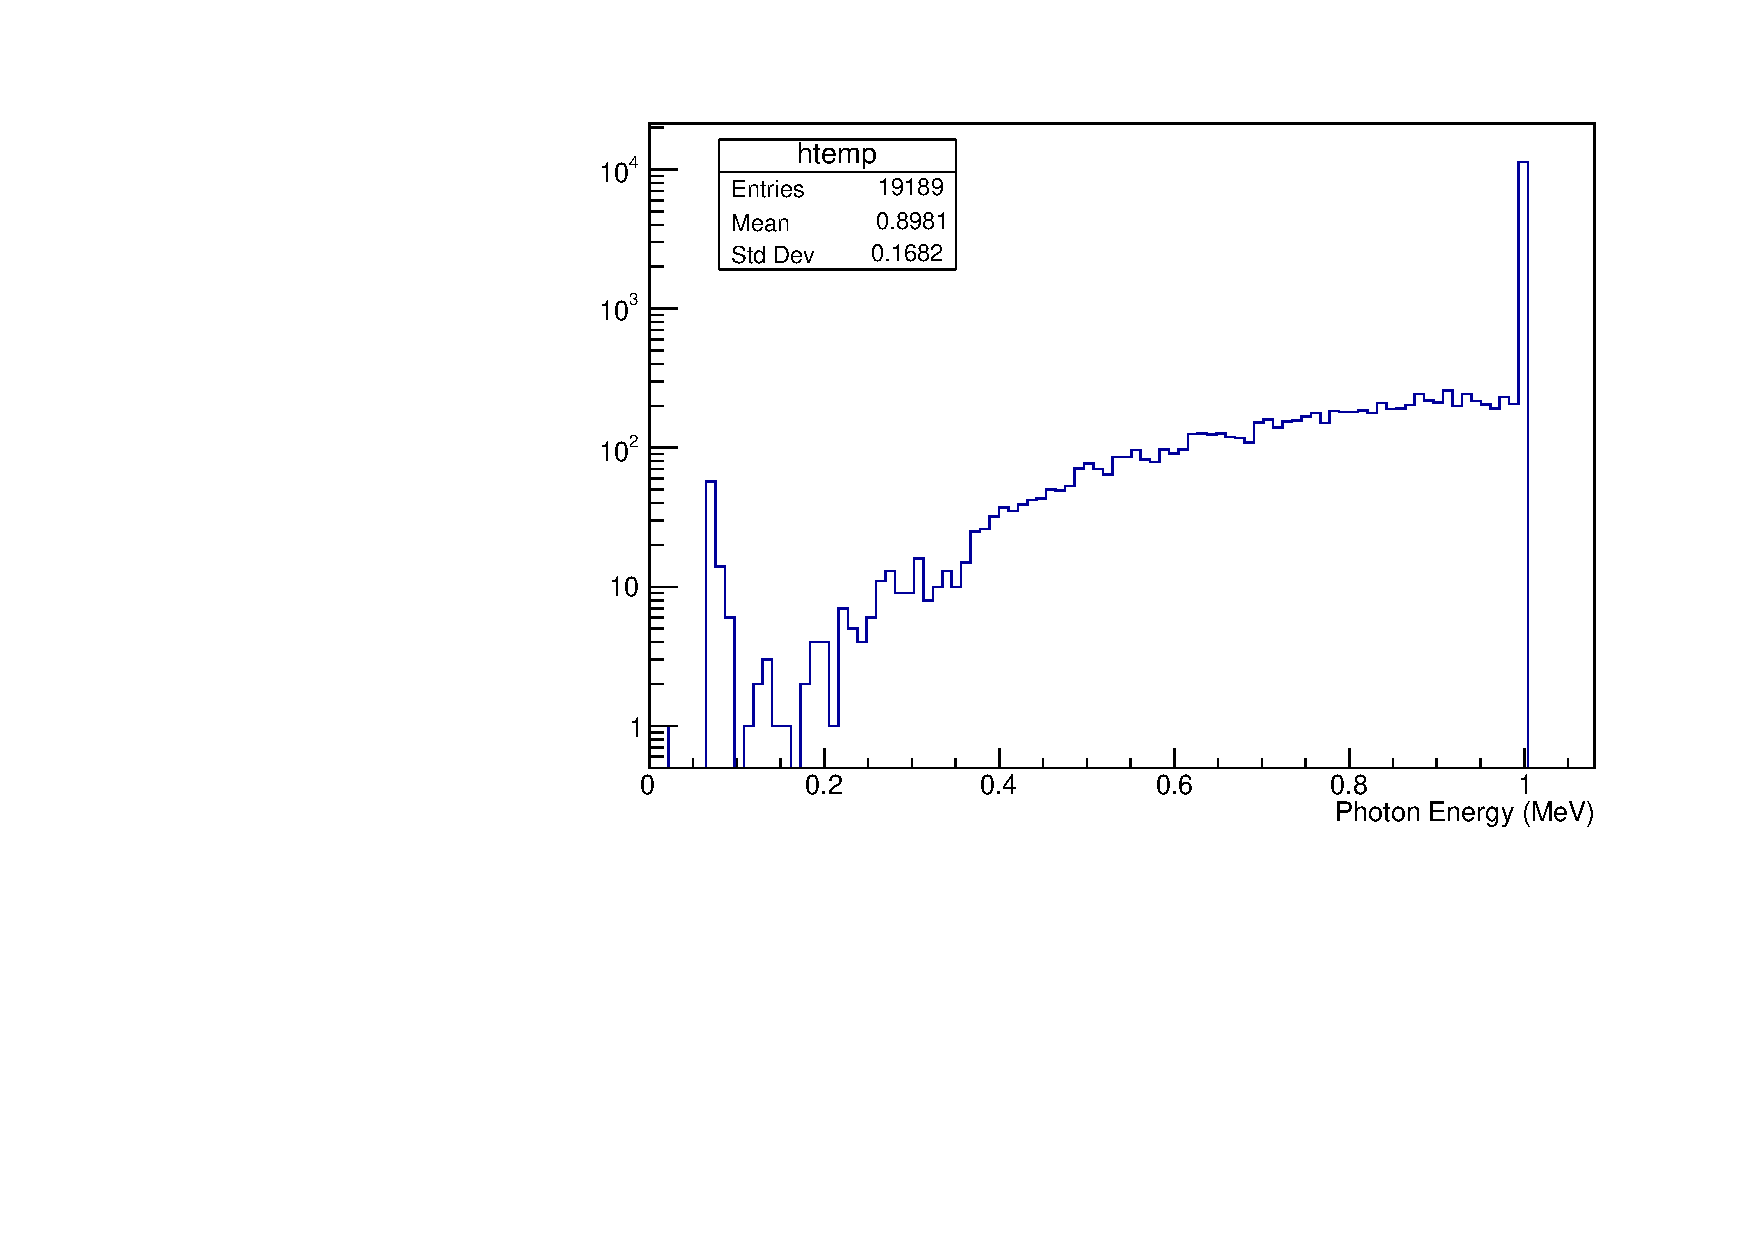
\includegraphics[width=0.5\linewidth]{energy_pop.pdf}
		\caption{Histograma da distribuição de energia das partículas detetadas.}
		\label{fig:energy_population}
	\end{figure}

	\paragraph{} Na distribuição de energia das partículas detetadas da Figura \ref{fig:energy_population}, podemos observar 2 populações: uma com 1 MeV, que corresponde às partículas que não interagiram com a placa de Pb, outra com energia inferior a 1 MeV que corresponde às partículas que sofreram espalhamento de Compton e foram detetadas à saída da placa de Pb.

	\paragraph{} Podemos observar o ângulo de dispersão destas partículas e a sua distribuição espacial nas Figuras \ref{fig:angular_dist} e \ref{fig:spacial_dist}.

	\begin{figure}[H]
		\centering
		\begin{minipage}{0.45\linewidth}
			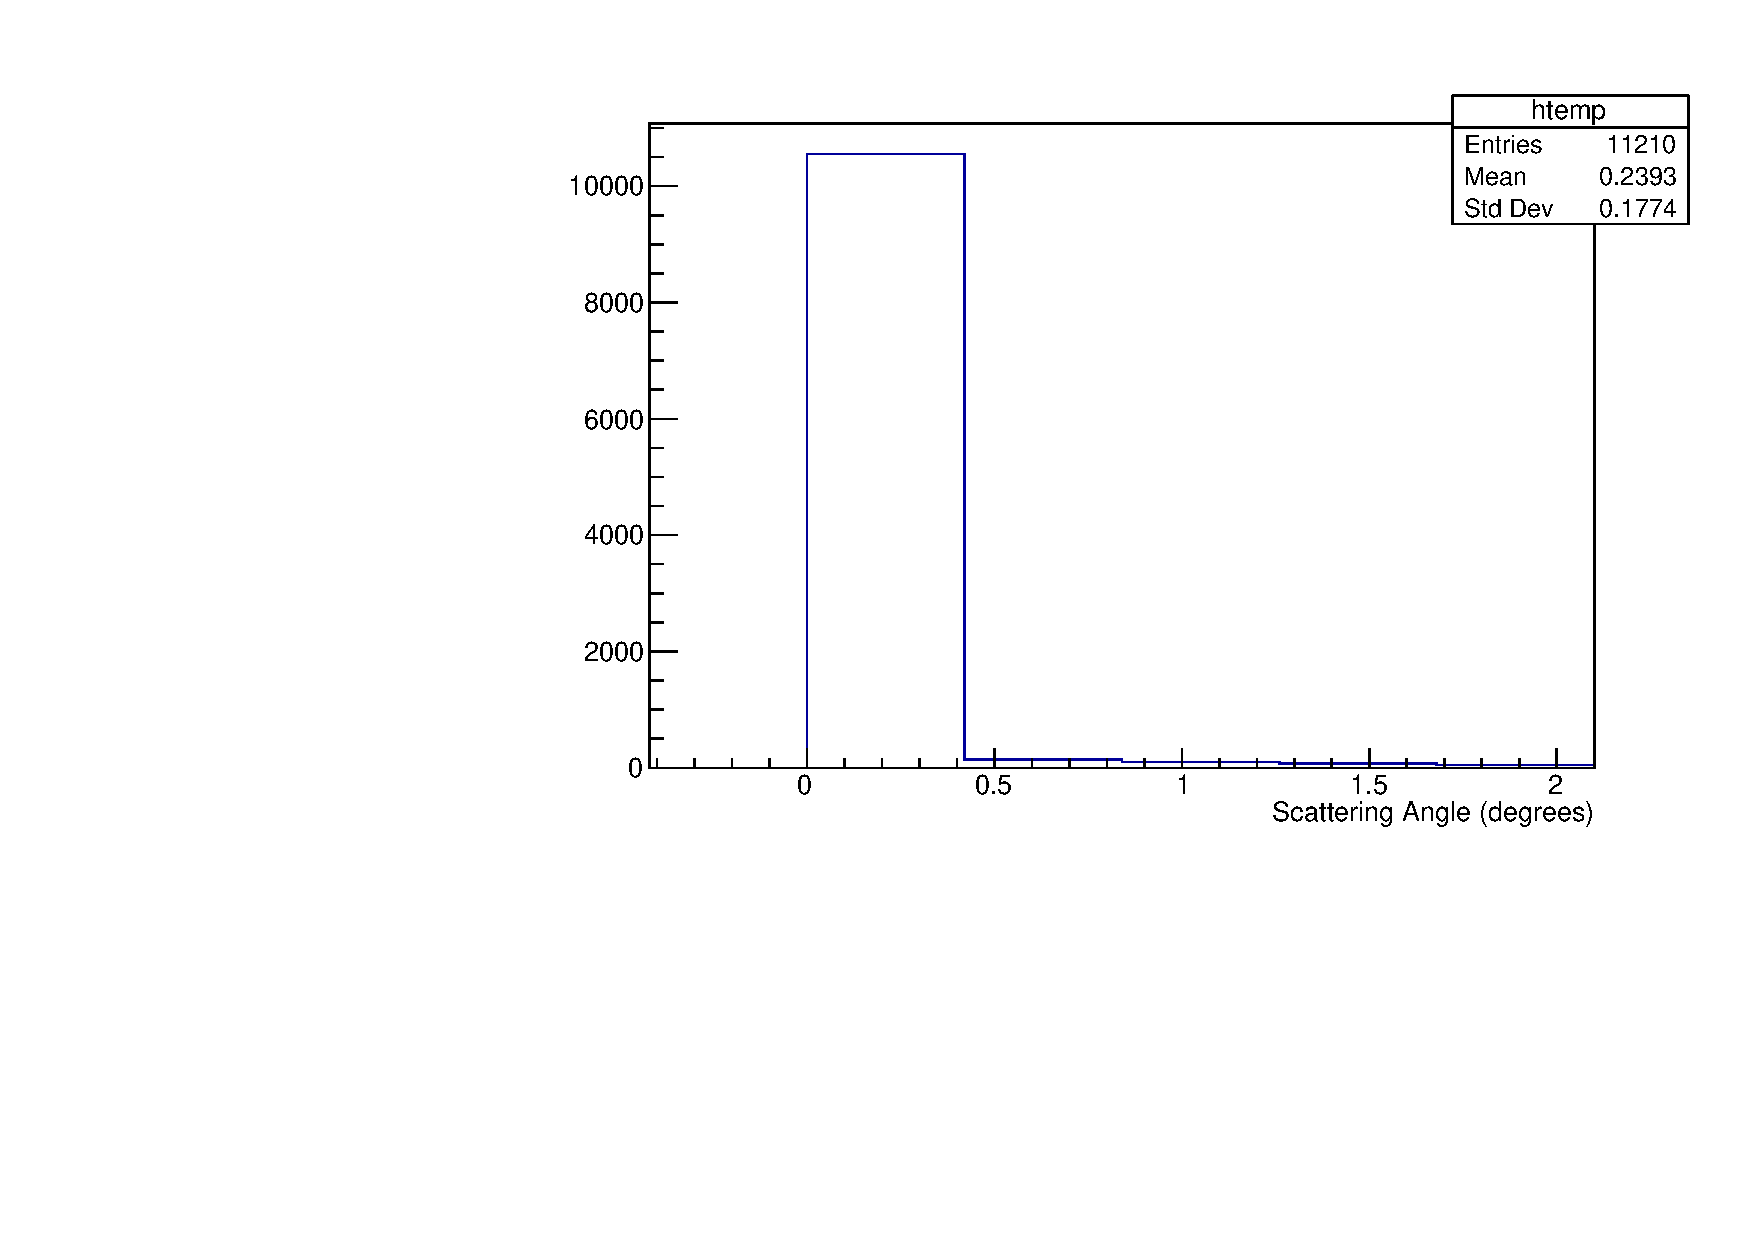
\includegraphics[width=\linewidth]{dist_pop_angle_1mev.pdf}
			\label{fig:angle_dist_inf1mev}
		\end{minipage}
		\begin{minipage}{0.45\linewidth}
			\centering
			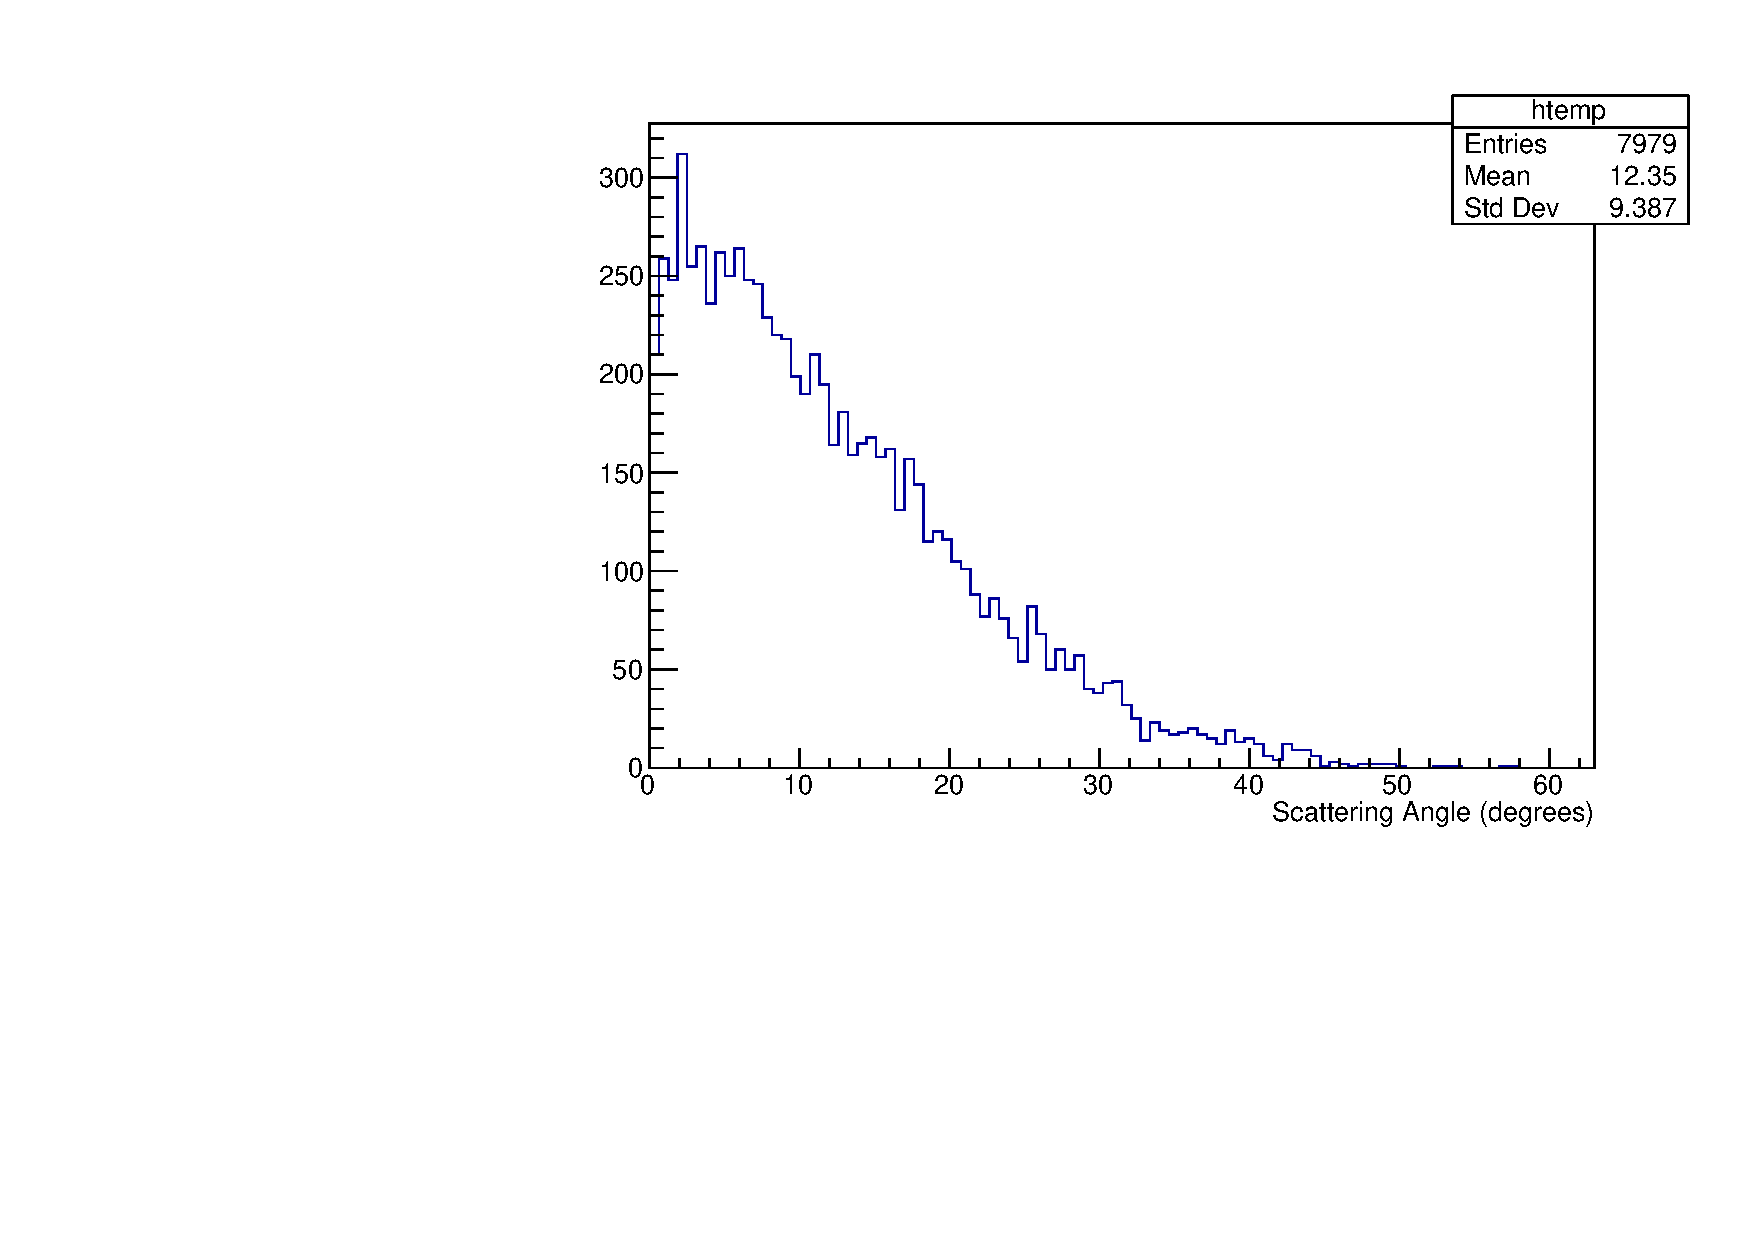
\includegraphics[width=\linewidth]{dist_pop_angle.pdf}
			\label{fig:angle_dist_1mev}
		\end{minipage}

		\caption{Histograma da distribuição angular das partículas detetadas. Para facilitar a análise, foram separadas as duas populações identificadas: à esquerda, temos a distribuição para partículas com energia igual a 1 MeV, à direita para partículas com energia inferior a 1 MeV.}
		\label{fig:angular_dist}
	\end{figure}


	\begin{figure}[H]
		\centering
		\begin{minipage}{0.45\linewidth}
			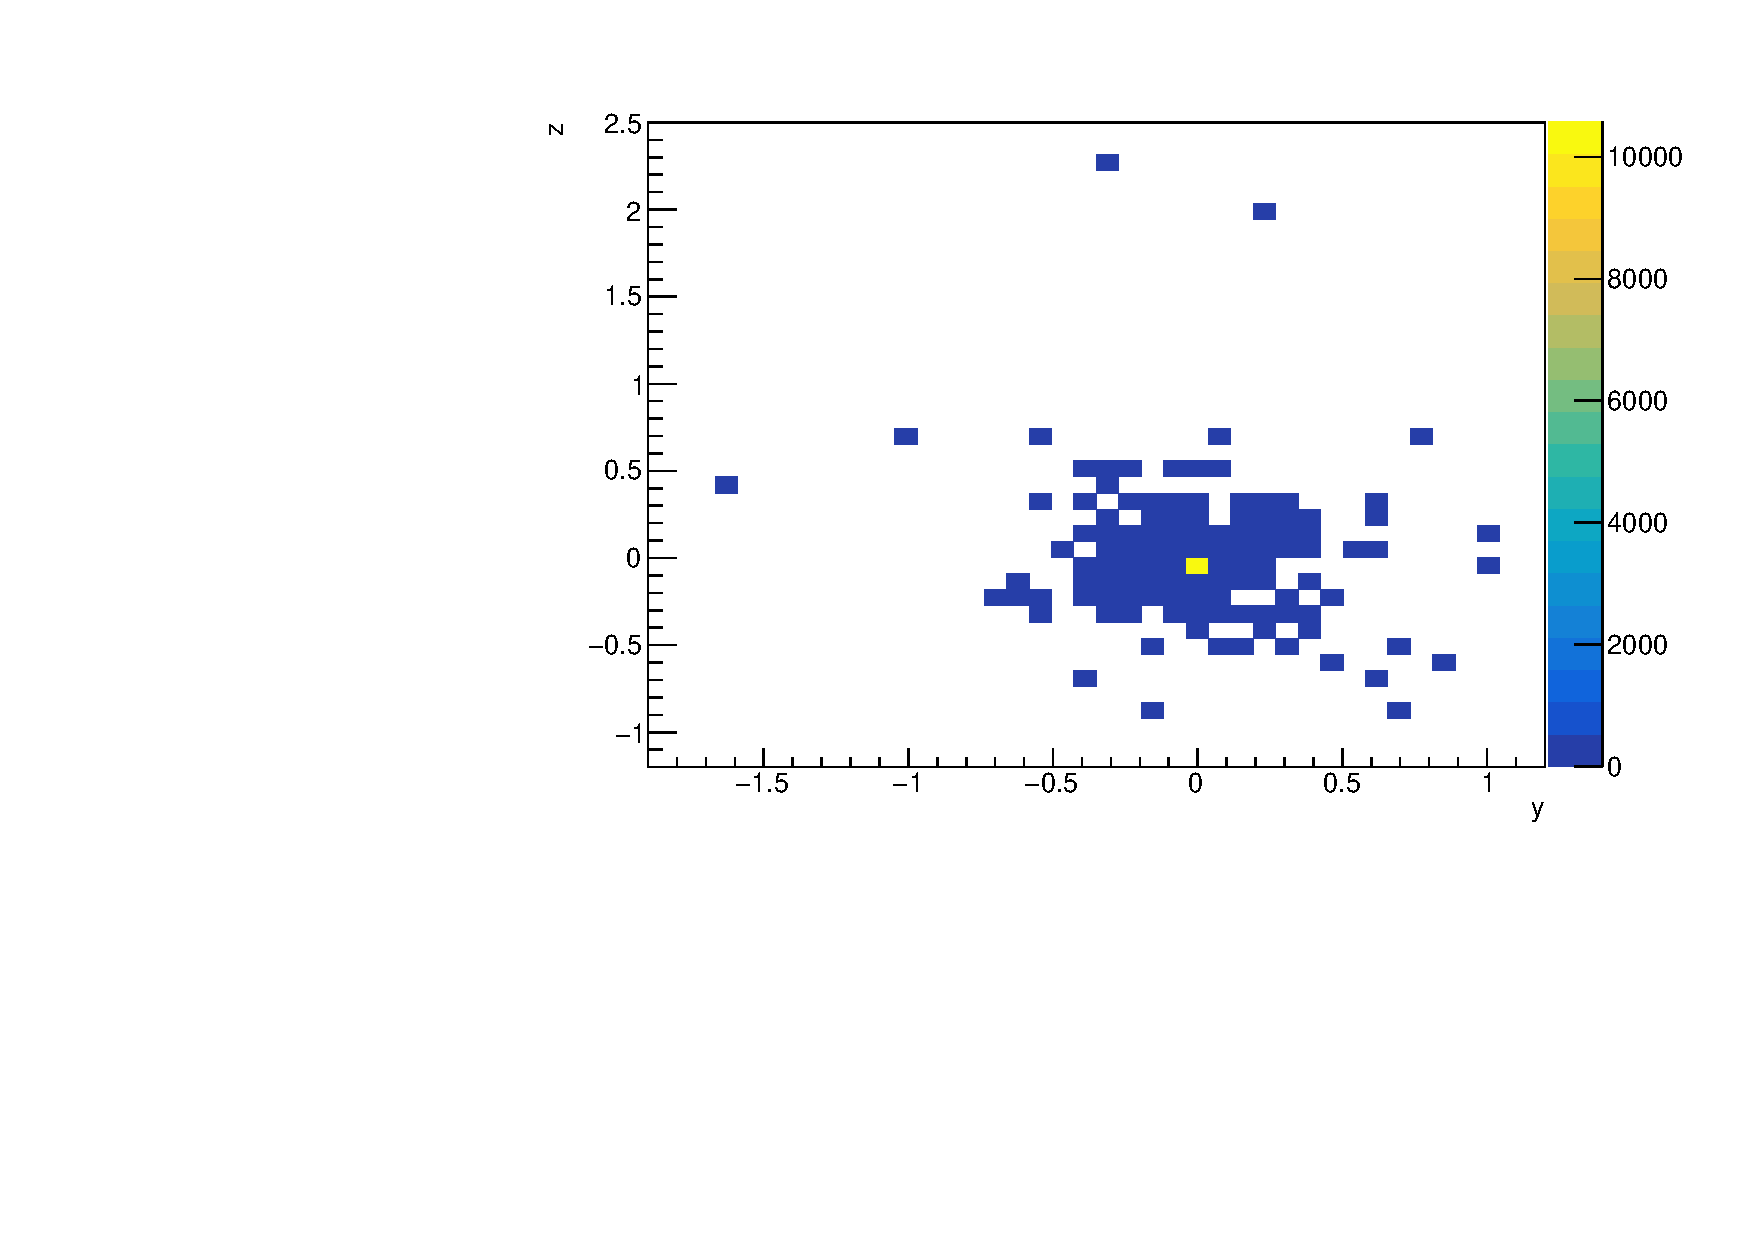
\includegraphics[width=\linewidth]{dist_zy_1mev.pdf}
			\label{fig:xy_dist_inf1mev}
		\end{minipage}
		\begin{minipage}{0.45\linewidth}
			\centering
			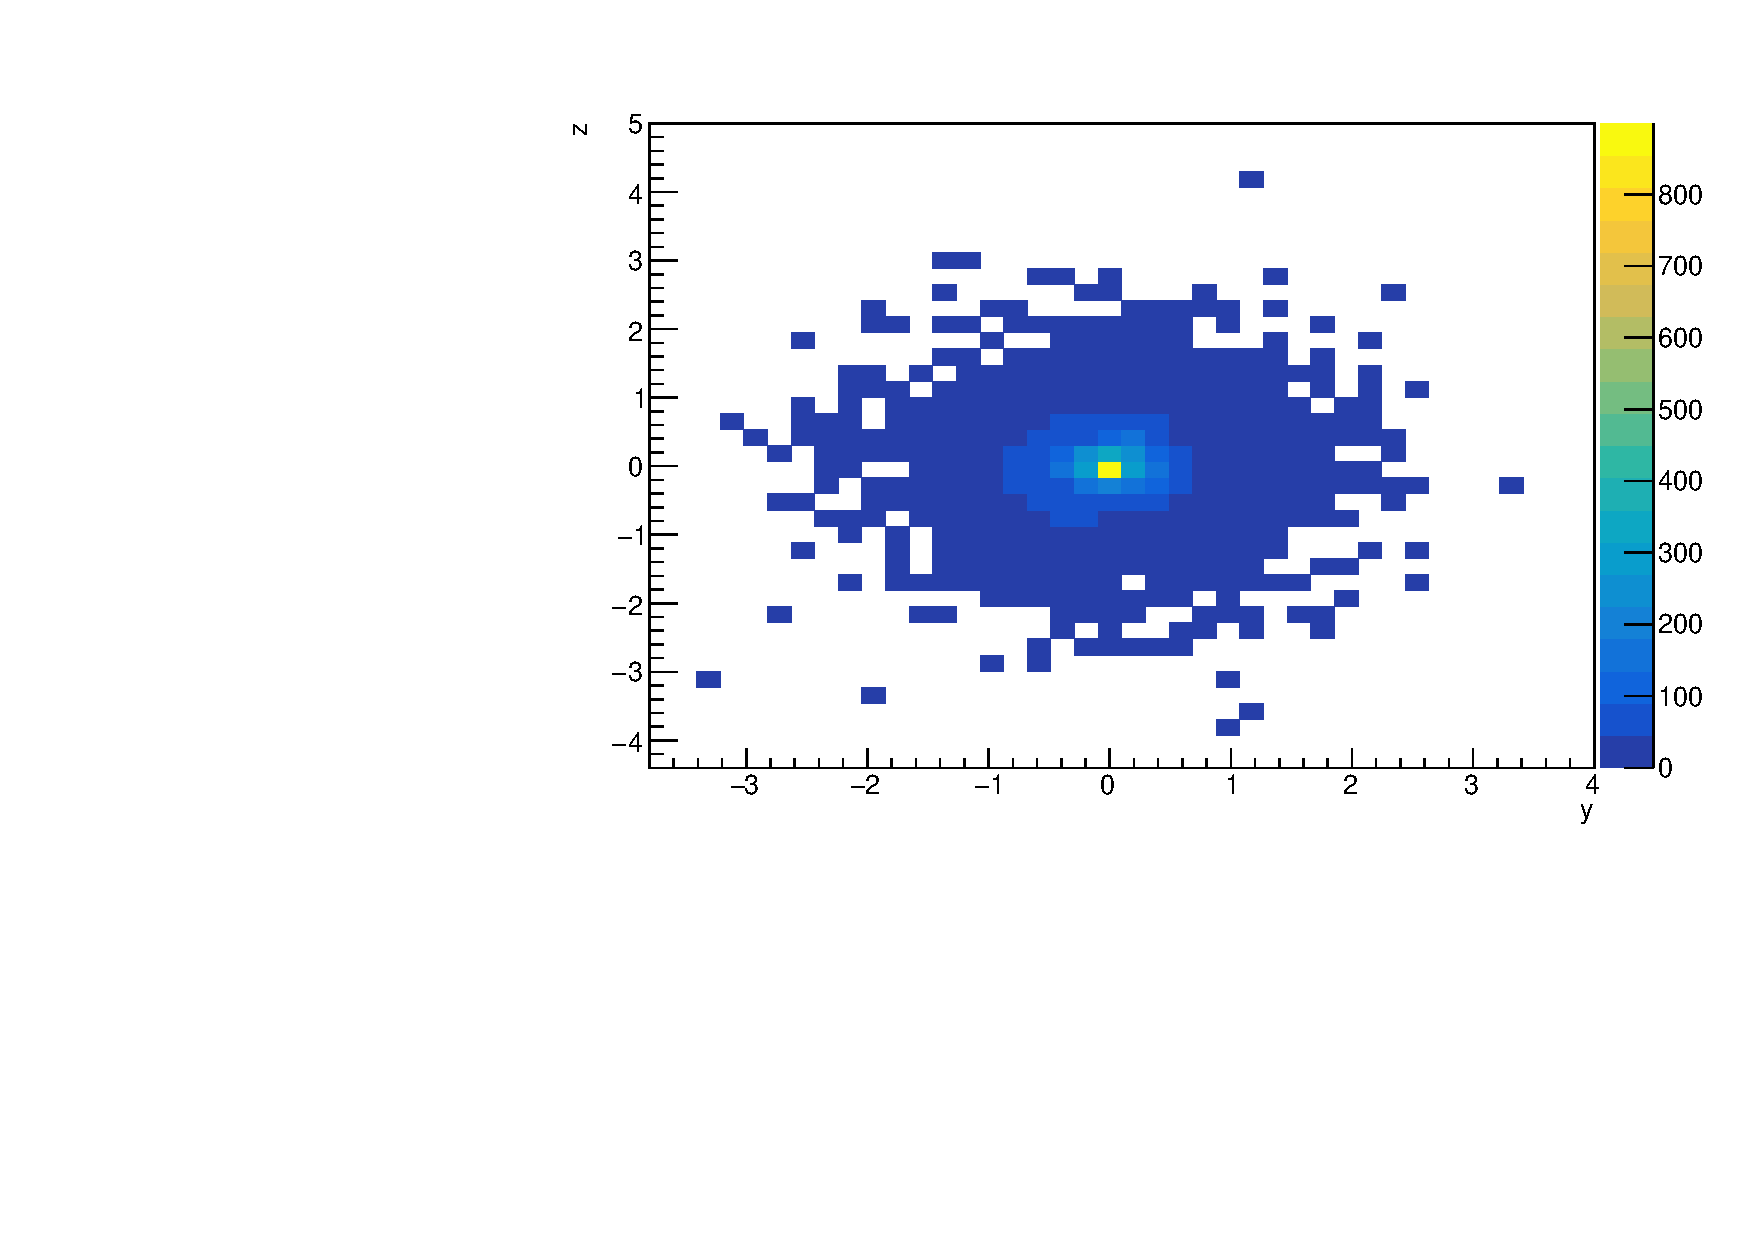
\includegraphics[width=\linewidth]{dist_zy_inf1mev.pdf}
			\label{fig:xy_dist_1mev}
		\end{minipage}

		\caption{Histograma da distribuição espacial das partículas detetadas à saída da placa de Pb. Para facilitar a análise, foram separadas as duas populações identificadas: à esquerda, temos a distribuição para partículas com energia igual a 1 MeV, à direita para partículas com energia inferior a 1 MeV.}
		\label{fig:spacial_dist}
	\end{figure}

\end{document}